\begin{frame}[t]{Funciones}\vspace{0pt}

Las funciones son \textit{procedimientos} que toman \underline{entradas} y producen \underline{salidas} (como una ``caja negra``). Los podemos utilizar una y otra vez a lo largo del código de programación.  

\begin{figure}
	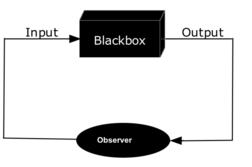
\includegraphics[scale=0.65]{Images/BlackBox.png}
\end{figure}

Las principales ventajas de las funciones son:

\begin{itemize}
	\item Mejora la lectura del código.
	\item Disminuye la escritura de líneas.
	\item Organiza los algoritmos.
\end{itemize}

\end{frame}